\begin{figure}[ht]
    \centering
    \begin{subfigure}{0.32\textwidth}
        \centering
        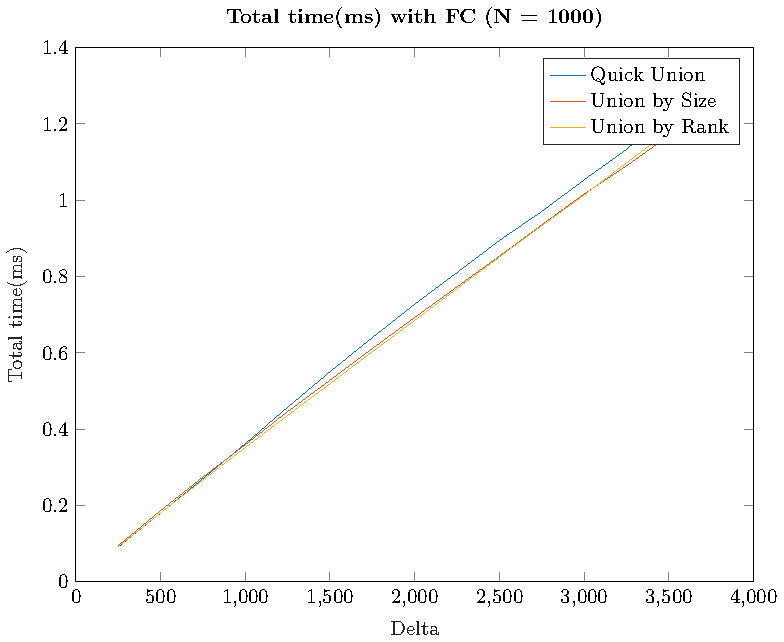
\includegraphics[width=\textwidth]{../images/plotFCFull1000_time(ms).pdf}
        \caption{Total Time with different union strategies with $n = 1000$ using Full Compression}
    \end{subfigure}%
    \hfill
    % Subfigure 2
    \begin{subfigure}{0.32\textwidth}
        \centering
        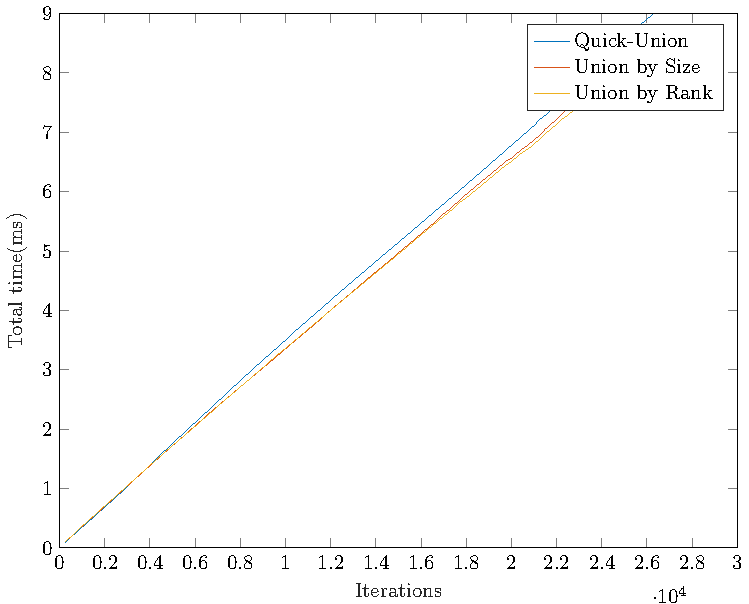
\includegraphics[width=\textwidth]{../images/plotFCFull5000_time(ms).pdf}
        \caption{Total Time with different union strategies with $n = 5000$ using Full Compression}
    \end{subfigure}%
    \hfill
    % Subfigure 3
    \begin{subfigure}{0.32\textwidth}
        \centering
        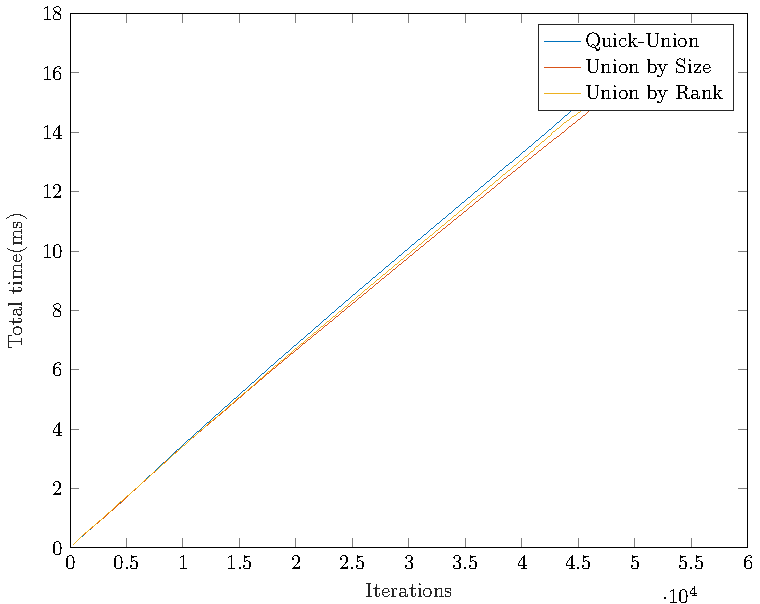
\includegraphics[width=\textwidth]{../images/plotFCFull10000_time(ms).pdf}
        \caption{Total Time with different union strategies with $n = 10000$ using Full Compression}
    \end{subfigure}
    % Subfigure 1
    \begin{subfigure}{0.32\textwidth}
        \centering
        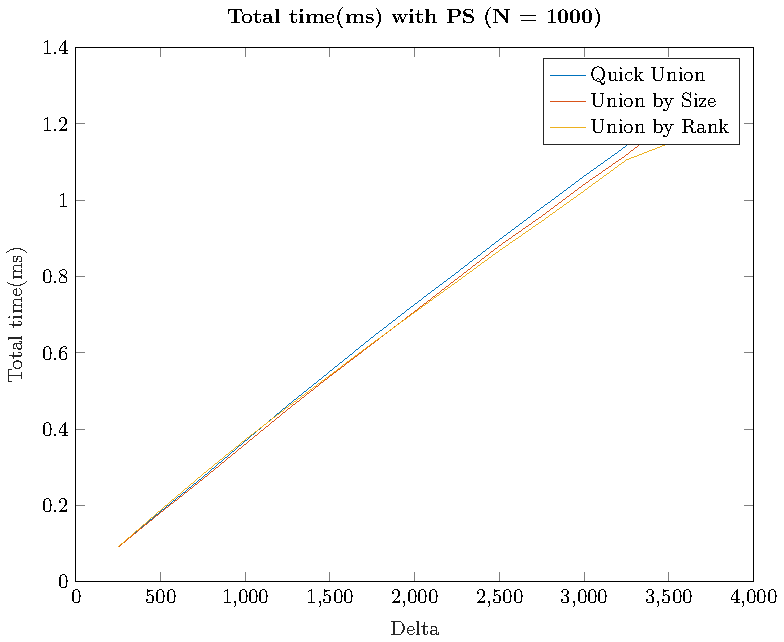
\includegraphics[width=\textwidth]{../images/plotPSFull1000_time(ms).pdf}
        \caption{Total Time with different union strategies with $n = 1000$ using Path Splitting}
    \end{subfigure}%
    \hfill
    % Subfigure 2
    \begin{subfigure}{0.32\textwidth}
        \centering
        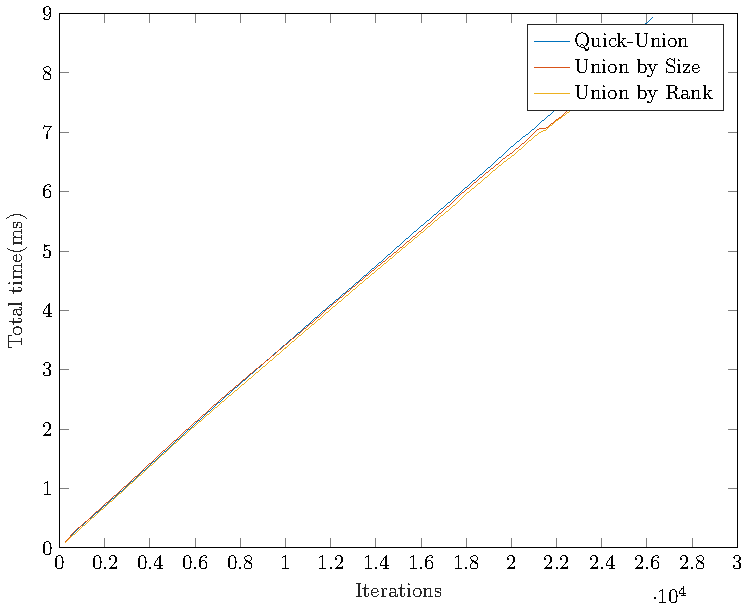
\includegraphics[width=\textwidth]{../images/plotPSFull5000_time(ms).pdf}
        \caption{Total Time with different union strategies with $n = 5000$ using Path Splitting}
    \end{subfigure}%
    \hfill
    % Subfigure 3
    \begin{subfigure}{0.32\textwidth}
        \centering
        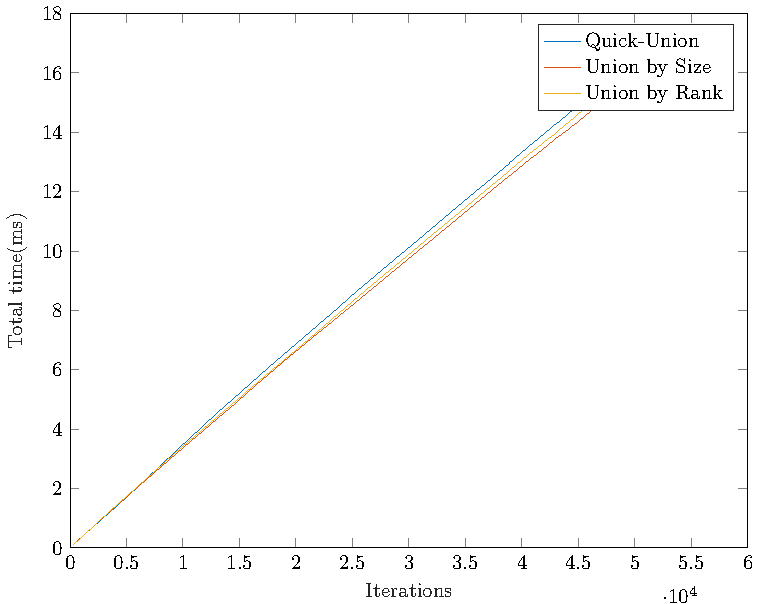
\includegraphics[width=\textwidth]{../images/plotPSFull10000_time(ms).pdf}
        \caption{Total Time with different union strategies with $n = 10000$ using Path Splitting}
    \end{subfigure}

    \begin{subfigure}{0.32\textwidth}
        \centering
        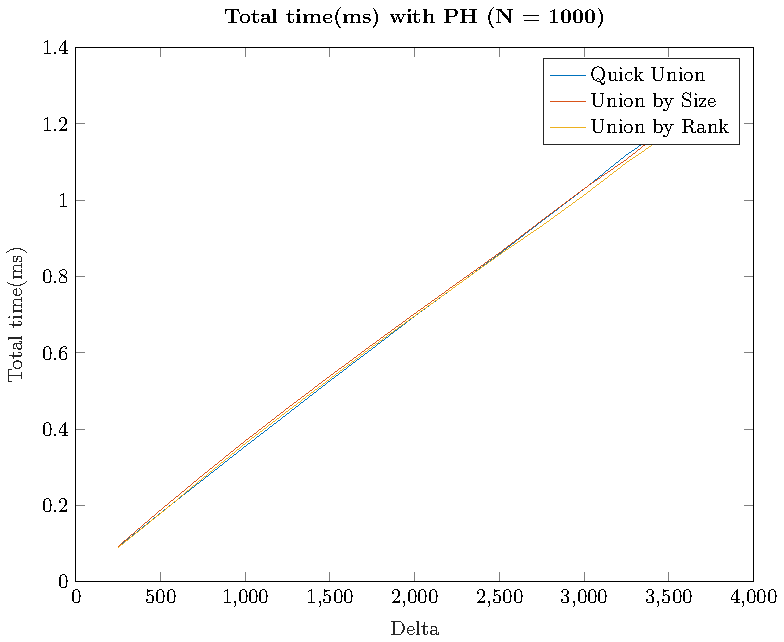
\includegraphics[width=\textwidth]{../images/plotPHFull1000_time(ms).pdf}
        \caption{Total Time with different union strategies with $n = 1000$ using Path Halving}
    \end{subfigure}%
    \hfill
    % Subfigure 2
    \begin{subfigure}{0.32\textwidth}
        \centering
        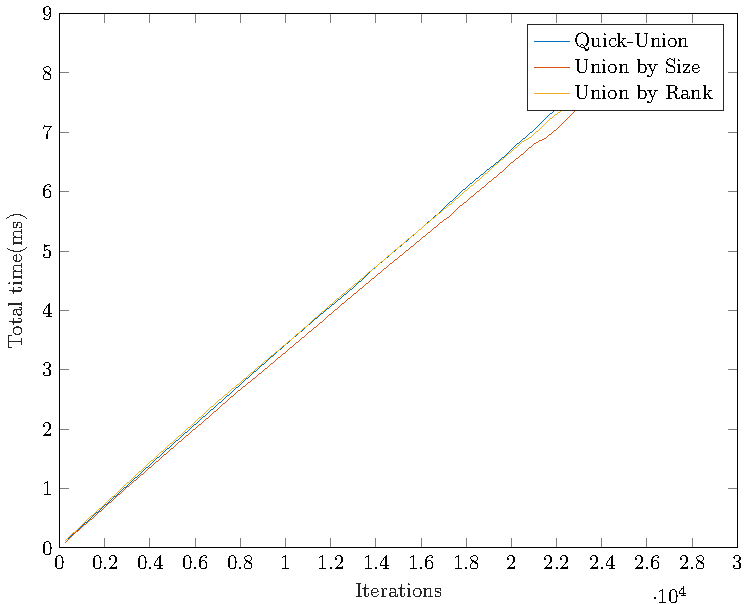
\includegraphics[width=\textwidth]{../images/plotPHFull5000_time(ms).pdf}
        \caption{Total Time with different union strategies with $n = 5000$ using Path Halving}
    \end{subfigure}%
    \hfill
    % Subfigure 3
    \begin{subfigure}{0.32\textwidth}
        \centering
        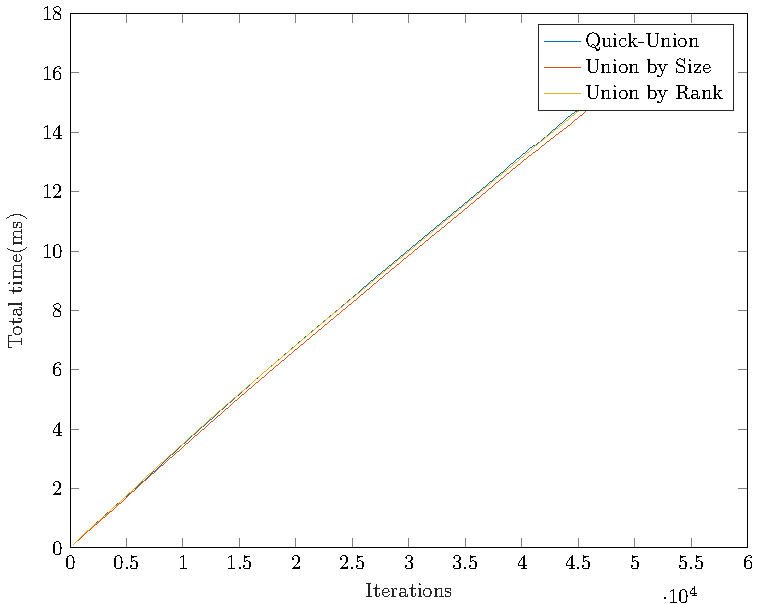
\includegraphics[width=\textwidth]{../images/plotPHFull10000_time(ms).pdf}
        \caption{Total Time with different union strategies with $n = 10000$ using Path Halving}
    \end{subfigure}
    \begin{subfigure}{0.32\textwidth}
        \centering
        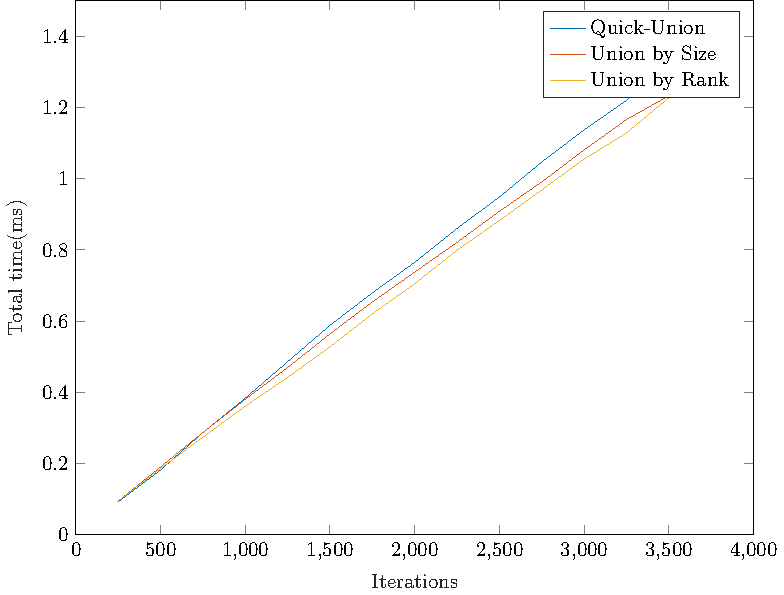
\includegraphics[width=\textwidth]{../images/plotTORFull1000_time(ms).pdf}
        \caption{Total Time with different union strategies with $n = 1000$ using Type One Reversal}
    \end{subfigure}%
    \hfill
    % Subfigure 2
    \begin{subfigure}{0.32\textwidth}
        \centering
        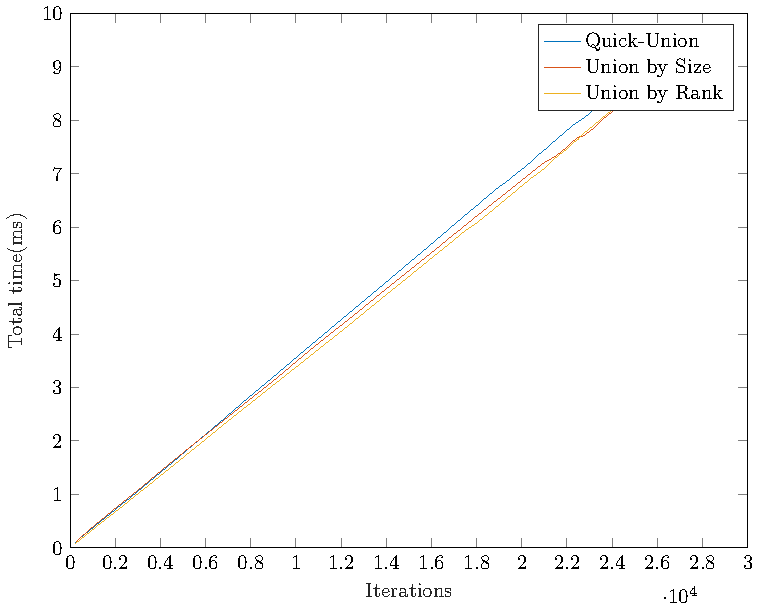
\includegraphics[width=\textwidth]{../images/plotTORFull5000_time(ms).pdf}
        \caption{Total Time with different union strategies with $n = 5000$ using Type One Reversal}
    \end{subfigure}%
    \hfill
    % Subfigure 3
    \begin{subfigure}{0.32\textwidth}
        \centering
        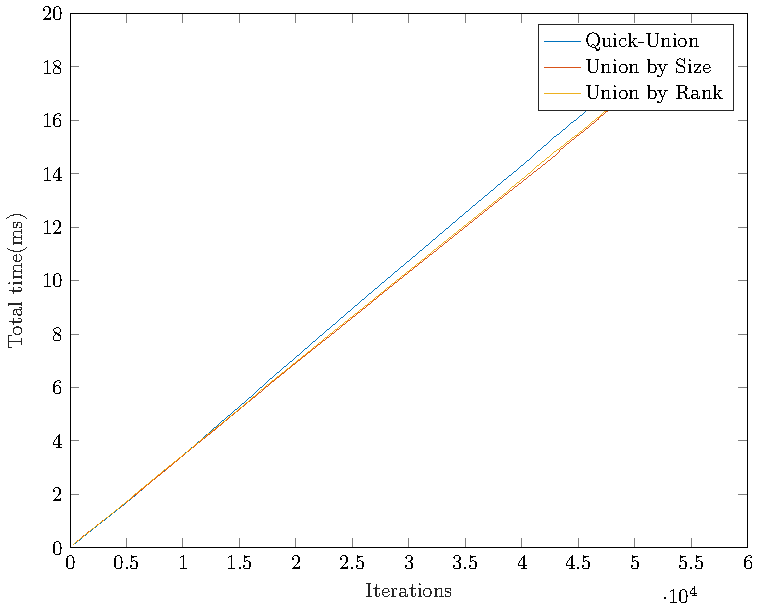
\includegraphics[width=\textwidth]{../images/plotTORFull10000_time(ms).pdf}
        \caption{Total Time with different union strategies with $n = 10000$ using Type One Reversal}
    \end{subfigure}

    \caption{Total time using different heuristics}
    \label{fig:timeH}
\end{figure}
